
An arbitrary reference to an astrophysics paper to demonstrate referencing. \citep{AasiAbadie2013}

\lipsum[1-2]

\section{A section}
\lipsum[5]
\begin{itemize}
\item Example of a list
\item It has two entries
\end{itemize}
\subsection{A subsection}
\lipsum[4]

\begin{figure}[h]
  \centering
  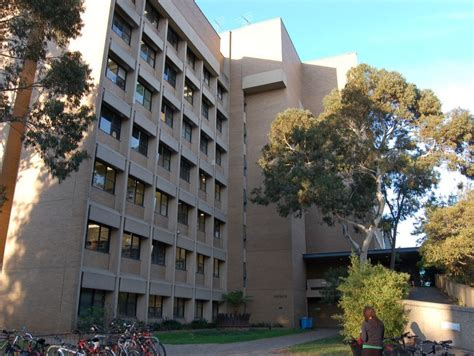
\includegraphics[width=0.9\linewidth]{figures/davidcaro.png}
  \caption{\label{fig:davidcaro} The asbestos tower of academia.}
\end{figure}

\lipsum[5-10]


